\documentclass[a4paper,10pt]{report}
\usepackage[utf8]{inputenc}
\usepackage{multirow}
\usepackage{graphicx}
\usepackage[margin=1.0in]{geometry}
\renewcommand\thesection{\arabic{section}}
\renewcommand\thesubsection{\thesection.\arabic{subsection}}

% Title Page
\title{Rendering and Compositing Infrastructure Improvements to VisIt for Insitu Rendering}
\author{Burlen Loring and Oliver Oliver R\"ubel}


\begin{document}
\maketitle

\begin{abstract}
Compared to posthoc rendering, insitu rendering often generates larger numbers of images, as a result rendering performance and scalability are critical in the insitu setting. In this work we present improvements to VisIt's rendering and compositing infrastructure that deliver increased performance and scalability in both posthoc and insitu settings. We added the capability for alpha blend compositing and use it with ordered compositing when datasets have disjoint block domain decomposition to optimize the rendering of transparent geometry. We also made improvements that increase overall efficiency by reducing communication and data movement and have addressed a number of performance issues. We structured our code to take advantage of SIMD parallelization and use threads to overlap communication and compositing. We tested our improvements on a 20 core workstation using 8 cores to render geometry generated from a $256^3$ cosmology dataset and on a Cray XC31 using 512 cores to render geometry generated from a $2000^2 \times 800$ plasma dataset. Our results show that ordered compositing provides a speed up of up to $4 \times$ over the current sort first strategy. The other improvements resulted in modest speed up with one notable exception where we achieve up to $40 \times$ speed up of rendering and compositing of opaque geometry when both opaque and transparent geometry are rendered together. We also investigated the use of depth peeling, but found that the implementation provided by VTK is substantially slower,both with and without GPU acceleration, than a local camera order sort.
\end{abstract}

\section{Introduction}
Insitu visualization and analysis seeks to reduce or eliminate data movement to and from disk by linking a simulation and a visualization run time using shared memory for data transfer. Insitu rendering has the potential for huge reductions in I/O costs as problem sized data is reduced to a single image before I/O. One potential drawback to insitu rendering is that one often doesn't know which fields will be interesting and which rendering parameters will produce the best result. For these reasons, compared posthoc rendering, insitu rendering generates a larger number of images, covering more fields, and wider array of rendering parameters. For these reasons rendering performance and scaling becomes a crucial issue in the insitu setting.

We profiled VisIt during 3D simulations of proton accelerator using WarpIV, an insitu visualization application that couples VisIt and Warp a laser plasma accelerator framework. Our profiling identified the rendering and compositing of translucent geometry as issues.

In this work we present optimizations and improvements to VisIt's rendering and compositing infrastructure. We added the capability for alpha blend compositing and use it with ordered compositing when datasets have disjoint block domain decomposition to increase performance when rendering transparent geometry. We also made improvements that increase overall efficiency and addressed a number of performance issues. We structured our code to take advantage of SIMD parallelization and use threads to overlap communication and compositing. We tested our work on a 20 core workstation using 8 cores to render geometry generated from a $256^3$ cosmology dataset and on a Cray XC31 using 512 cores to render geometry generated from a $2000^2 \times 800$ plasma dataset. Our results show that ordered compositing provides a speed up of up to $4 \times$ over the current sort first strategy. The other improvements resulted in modest speed up with one notable exception where we achieve up to $40 \times$ speed up of rendering and compositing of opaque geometry when both opaque and transparent geometry are rendered together. We also investigated the use of depth peeling, but found that the implementation provided by VTK is substantially slower,both with and without GPU acceleration, than a local camera order sort.

\section{Description of the Work}
Prior to our work VisIt always used a ``sort first'' strategy for rendering transparent geometry in parallel. In this strategy prior to rendering data was moved using MPI such that each process had all the geometry covered by a screen space tile. After rendering each process sends its tile to rank 0 for assemblage. In this arrangement one can apply serial rendering algorithms, and alpha blend compositing is not necessary. This is illustrated in figure \ref{fig:example}. On the left a dataset with 10 iso-surfaces is shown. The coloring by MPI rank id reveals the block based domain decomposition. In the sort first strategy, prior to rendering, the transparent geometry is moved to the screen space domain decomposition shown on the right. In what follows we refer to this data movement as a ``global sort''. The global sort is expensive because all of the data may need to be moved and it doubles the amount of memory used to store transparent geometry.

Our work builds on VisIt svn rev 27127(9/9/2015). We used rev 27127 as the baseline to compare our optimizations against. Parallel rendering in VisIt occurs in two logical passes, a pass for opaque geometry, and a pass for transparent geometry. Prior to our work, the opaque pass included a depth based composite where the unsigned char r,g,b color channels and float depth values are packed into an AOS(array of structures) layout and composited in user defined MPI reduction operation; and the transparent pass included a distributed global geometry sort which moves data onto a decomposition such that each rank ends up with geometry for a unique screen space tile, followed by a local camera order sort and render, followed by an MPI gather of each ranks tile to rank 0.

Our work extended the transparent rendering and compositing capabilities of VisIt in four main ways: 
\begin{itemize}
 \item We implemented an alpha blending compositer and a depth based compositer. Our new compositer operates on SOA(structures of arrays) data layout to make use of compiler auto-vectorization. We used threads to overlap communication and compositing. We arranged the communications in a binary tree pattern but also made provision for supporting a variety of alternative communication patterns.
 \item We implemented the ordered compositing optimization, which for translucent block domain decomposed data eliminates the communication associated with the global sort and cuts memory overhead in half.
 \item We added the capability to enable VTK's depth peeling algorithm from VisIt's GUI.
 \item We optimized code, cleaned up, and fixed bugs as we went.
\end{itemize}

\section{Optimizations}
\subsection*{Ordered Compositing}
\begin{figure}
\centering
\begin{minipage}{0.48\textwidth}
\begin{center}
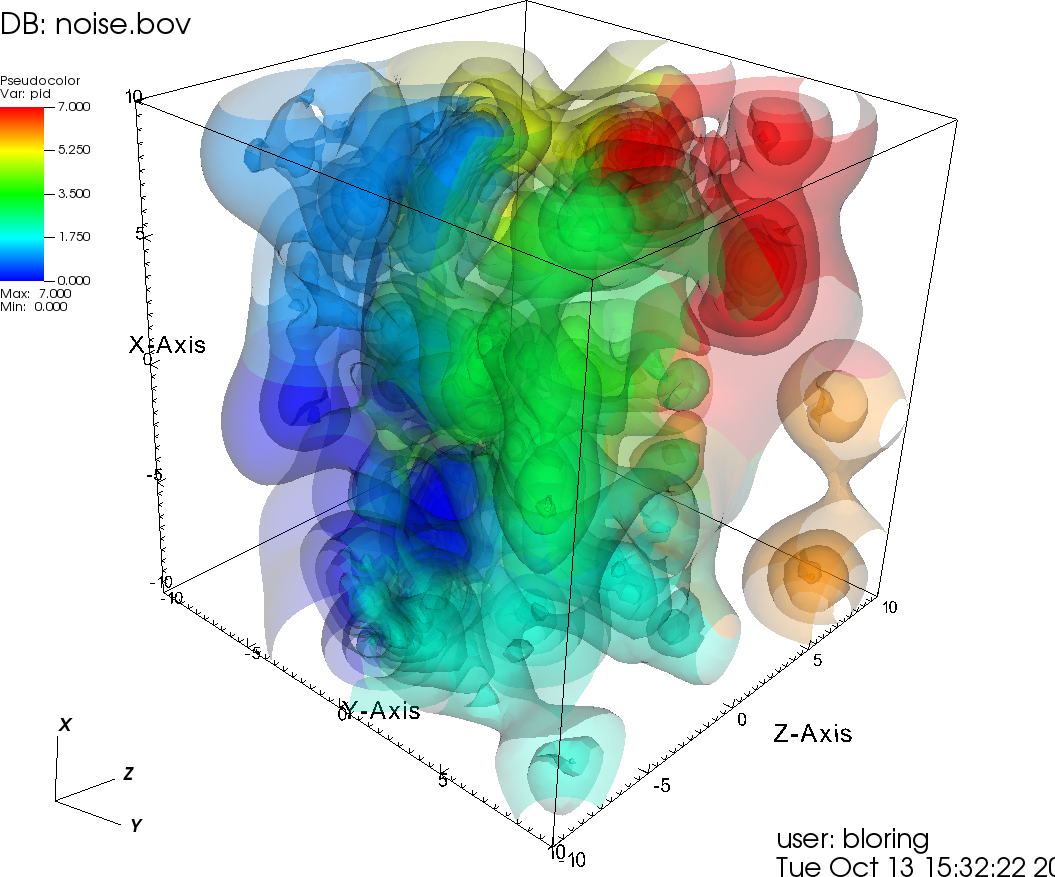
\includegraphics[height=2.5in]{./order_composite_example_color.png}
\end{center}
\end{minipage}
\begin{minipage}{0.48\textwidth}
\begin{center}
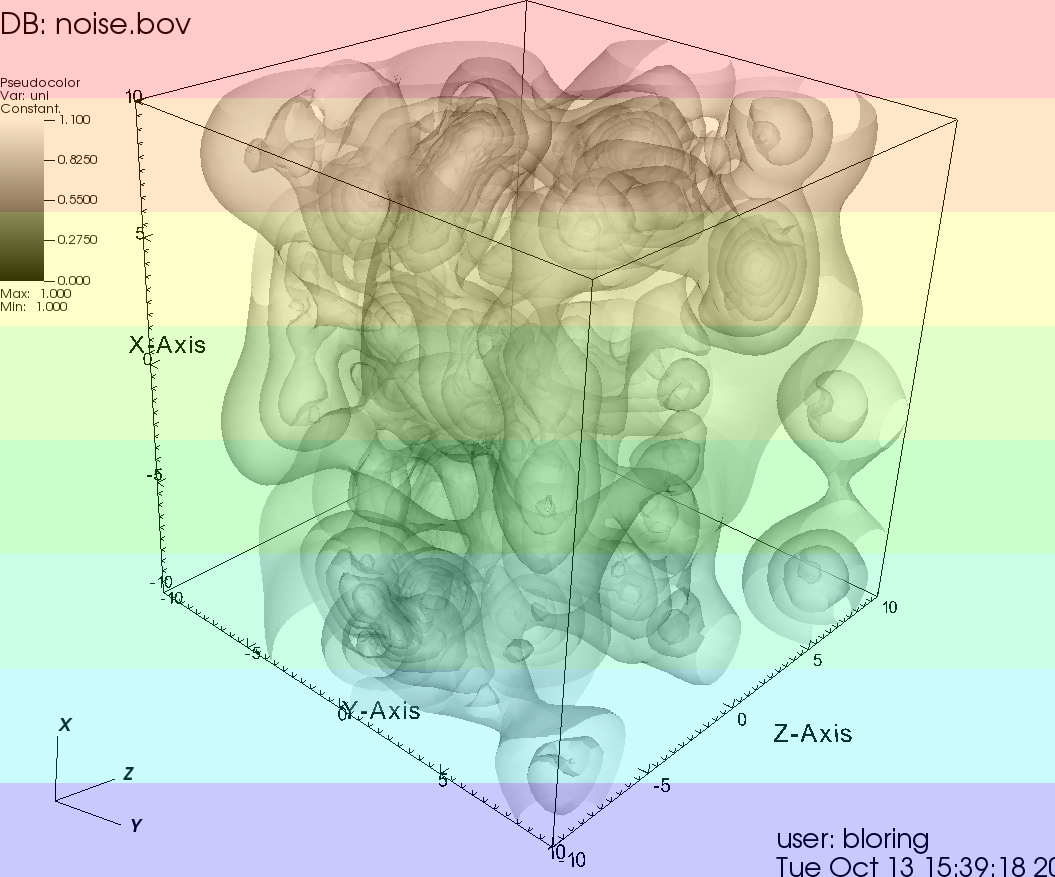
\includegraphics[height=2.5in]{./tiled_image_example_color.png}
\end{center}
\end{minipage}
\begin{minipage}{0.55\textwidth} 
\caption{\footnotesize Ordered compositing and image tiled compositing example. The original domain decomposition is shown on the left. Ordered compositing renders the data using this decomposition. The tiled image compositing decomposition is shown on the right. Tiled compositing moves data to that decomposition prior to rendering.}
\label{fig:example}
\end{minipage}\hspace{0.04in}
\begin{minipage}{0.3\textwidth}
{\footnotesize
\def\arraystretch{1.25}
\begin{tabular}{|ll|}
\multicolumn{2}{c}{} \\ \hline
\multicolumn{2}{|c|}{\bf composite order = 4 5 6 0 7 1 2 3} \\ \hline
round 0: & $4 \leftarrow 5, 6 \leftarrow 0, 7 \leftarrow 1, 2 \leftarrow 3$  \\
round 1: & $4 \leftarrow 6, 7 \leftarrow 2$  \\
round 2: & $4 \leftarrow 7$ \\ \hline
\end{tabular}}
\end{minipage}
\end{figure}

Ordered compositing is an optimization for rendering translucent block decomposed data. When the decomposition's block's bounds are mutually disjoint one can find a compositing order that produces the same result as a global sort without moving any data. Compared to the sort-first strategy rather than re-distributing geometry in a global sort, ordered compositing renders the data in place and uses alpha bend compositing to combing each processes rendering. Ordered compositing is faster when the amount of data to move in the global sort is large. An example is shown in figure \ref{fig:example}. The data is rendered using the domain decomposition shown on the left. Our alpha blending compositer makes use of associativity of the alpha blending operation and structures the compositing in a binary tree. The compositing order and subsequent tree is shown in the table in figure \ref{fig:example}. When the root of the tree is not rank 0, the final image needs to be transferred to rank 0.

\subsection*{Other Improvements}
The main optimization is ordered compositing. We investigated the following other optimizations:
\begin{itemize}
 \item SIMD vectorization of the depth and blending compositer kernels
 \item using threads to overlap communication and compositing
 \item eliminating memcpy where ever possible, including making better use of shallow copy of VTK objects
 \item eliminate read-back from OpenGL if not using the channel
 \item eliminating or reducing communication where ever possible
 \item only update sorting pipeline when dependent input parameters change
\end{itemize}

\section{Results}
We benchmarked our work on two datasets, a $256^3$ cosmology simulation and a $2000^2 \times 800$ plasma simulations, on two systems, a 20 core graphics workstation using 8 cores and a Cray XC31 using 512 cores. The details can be found in the tables in figures \ref{fig:speedup_cosmo} and \ref{fig:speedup_vpic}. Our primary optimization, ordered compositing, generally produced substantial speed up. The results are dependent on the geometry size and the number of processes used. In our tests we achieved $\approx 2 \times$ speed up on the workstation and $\approx 4 \times$ speed up on the Cray. In general for the opaque pass our other optimizations achieved modest speed-up of on the order of 10\%. One notable exception is that when both rendering passes were engaged, during the opaque pass we achieved $\approx 11 \times$ speed up on the workstation, and $\approx 40 \times$ speed-up on the Cray. This is due to a bug we fixed that was causing the translucent geometry to be sorted(global+local) twice.

\begin{figure}[ht]
\centering
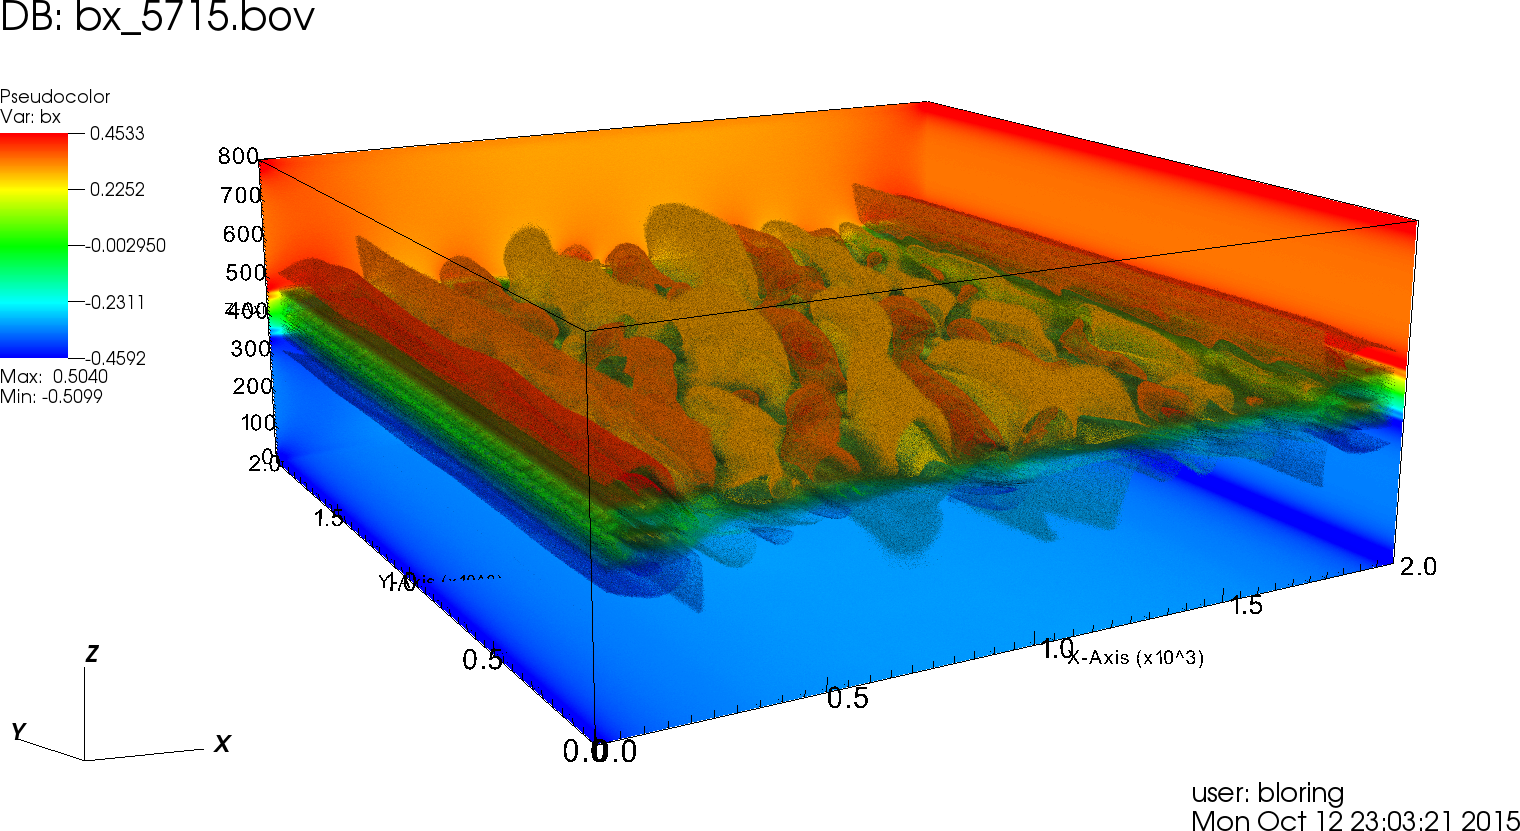
\includegraphics[height=3.0in]{./vpic_test_case_0030.png}
\begin{minipage}[c]{0.46\textwidth}
\begin{center}
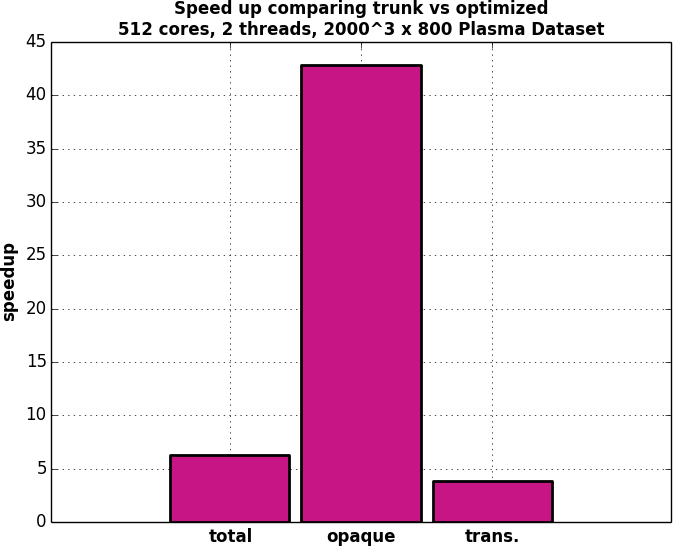
\includegraphics[height=2.25in]{./speed_up_vpic.png} 
\end{center}
\end{minipage}
\begin{minipage}{0.5\textwidth}
%\begin{center}
{\footnotesize
\def\arraystretch{1.25}
\begin{tabular}{|l|l|l|}
\hline
\multicolumn{3}{|c|}{\bf{Data rendered, Plasma}} \\ \hline
{\bf type} & {\bf desc.} & {\bf zones} \\ \hline
opaque & 3 slice &  7190403 \\ \hline
trans. & 20 iso & 464815961 \\ \hline
\end{tabular}}%
\hspace{-0.1in}{\footnotesize
\def\arraystretch{1.25}
\begin{tabular}{|c|c|}
\hline
\multicolumn{2}{|c|}{\bf{Speedup vs trunk}} \\ \hline
 total & 6.31 \\ \cline{1-2}
 opaque & 42.85 \\ \cline{1-2}
 transparent & 3.82 \\ \hline
\end{tabular}}\vspace{0.08in}
{\footnotesize
\def\arraystretch{1.5}
\begin{tabular}{|l|l|r|r|r|}
\hline
\multicolumn{5}{|c|}{\bf Render and Composite Time} \\ \hline
{\bf code} & {\bf configuration} & {\bf total} & {\bf trans.} & {\bf opaque} \\ \hline
\multirow{2}{*}{opt.} & global sort & 21.0305 & 20.6666 & 0.354182 \\ \cline{2-5}
 & ordered comp. &  6.01573 & 5.44624 & 0.400792 \\ \hline
trunk & global sort & 37.9864 & 20.8121 & 17.1737 \\ \hline
\end{tabular}}
%\end{center}
\end{minipage}
\caption{\footnotesize {\bf Top:} $2000^2 \times 800$ plasma dataset {\bf Bottom Left:} Speedup of rendering and compositing using 512 cores, and 2 threads, on the $2000^2 \times 800$ plasma dataset. Total and per pass time are shown. In the opaque pass z-buffer compositing is used while in the transparent pass ordered compositing and alpha blending are used. {\bf Bottom Right:} Data and measurements.}
\label{fig:speedup_vpic}
\end{figure}

\begin{figure}
\begin{minipage}{0.56\textwidth}
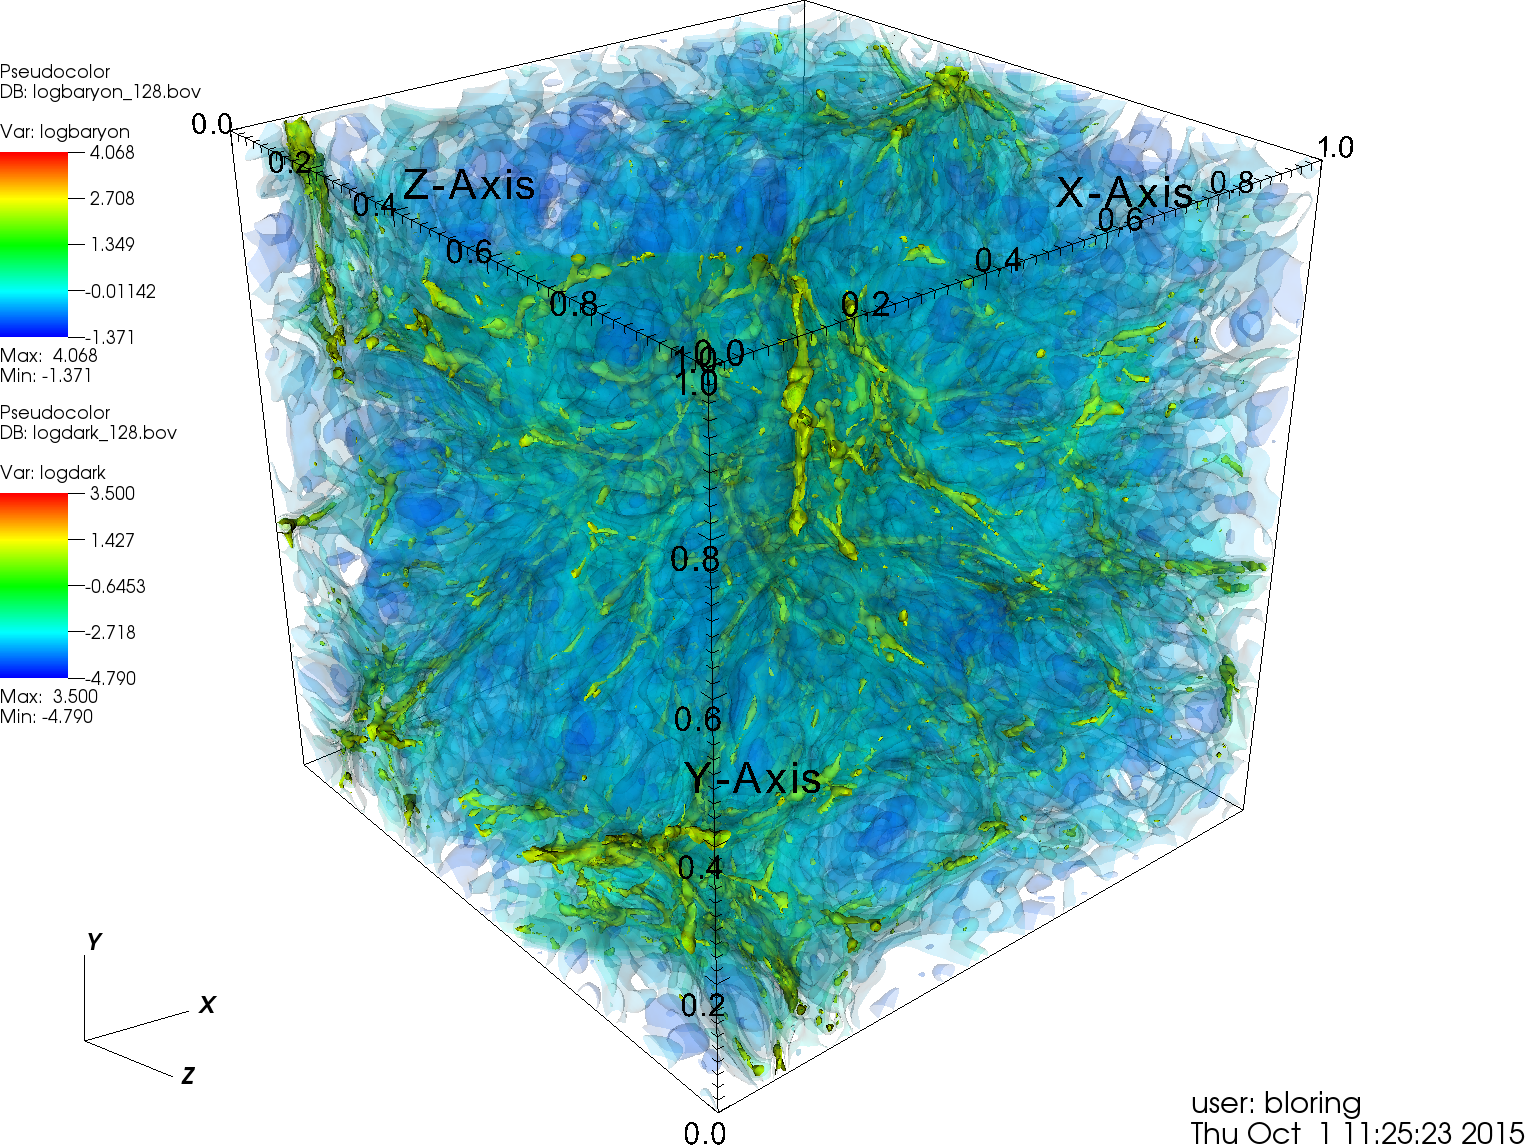
\includegraphics[height=3.0in]{./cosmology_test_case_0080.png} 
\end{minipage}
\begin{minipage}{0.30\textwidth}
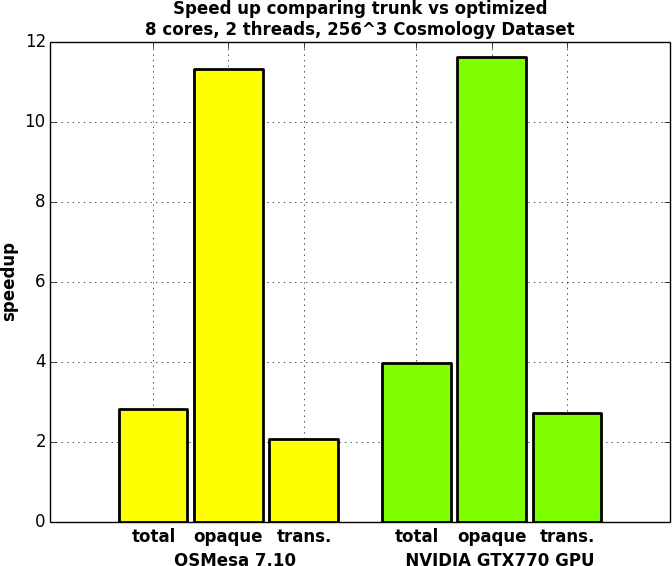
\includegraphics[height=2.25in]{./speed_up_cosmo.png} 
\end{minipage}

\begin{minipage}{1.0\textwidth}
\begin{center}
\vspace{0.05in}
{\footnotesize
\def\arraystretch{1.25}
\begin{tabular}{|l|l|l|}
\hline
\multicolumn{3}{|c|}{\bf{Cosmology data rendered}} \\ \hline
{\bf type} & {\bf desc.} & {\bf num zones} \\ \hline
opaque & 1 iso & 488520 \\ \hline
trans. & 10 iso & 9884369 \\ \hline
\end{tabular}} \vspace{0.05in}
\def\arraystretch{1.25}
{\footnotesize
\begin{tabular}{|c|c|c|}
\hline
\multicolumn{3}{|c|}{\bf{Speedup compared to trunk}} \\ \hline
\multirow{4}{*}{GTX770} & total & 3.58 \\ \cline{2-3}
 & opaque & 11.89 \\ \cline{2-3}
 & transparent & 2.34 \\ \hline
\multirow{3}{*}{OSMesa} & total & 2.83 \\ \cline{2-3}
 & opaque & 11.34 \\ \cline{2-3}
 & transparent & 2.08 \\ \hline
\end{tabular}}
\end{center}
\end{minipage}

\begin{minipage}{1.0\textwidth}
\begin{center}
{\footnotesize
\def\arraystretch{1.25}
\begin{tabular}{|l|l|l|l|l|l|l|l|}
\hline
\multicolumn{8}{|c|}{\bf Render and Composite Time, Cosmology} \\ \hline
\multicolumn{2}{|c|}{}& \multicolumn{3}{|c|}{\bf OSMesa 7.10 } & \multicolumn{3}{|c|}{\bf NVIDIA GTX770 GPU} \\ \hline
{\bf code} & {\bf configuration} & {\bf total} & {\bf trans.} & {\bf opaque} & {\bf total} & {\bf trans.} & {\bf opaque} \\ \hline
\multirow{3}{*}{opt.} & global sort &  4.30541 & 4.11388 & 0.187808 & 2.51254 & 2.33435 & 0.174466 \\ \cline{2-8}
 & ordered comp. & 2.16096 & 1.93264 & 0.184575 & 1.21876 & 1.00458 & 0.168962 \\ \cline{2-8}
 & depth peel & 42.0545 & 41.8255 & 0.185432 & 6.2353 & 6.02038 & 0.170824 \\ \hline
trunk & global sort &  6.11546 & 4.02224 & 2.09239 & 6.11546 & 4.02224 & 2.09239 \\ \hline
\end{tabular}}
\end{center}
\end{minipage}

\caption{\footnotesize {\bf Top Left:} $256^3$ cosmology dataset. {\bf Top Right:} Speedup of total rendering and compositing time using 8 cores, and 2 threads, on the $256^3$ cosmology dataset. Total and per pass time are shown. In the opaque pass z-buffer compositing is used while in the transparent pass ordered compositing and alpha blending are used. {\bf Bottom:} Data and measurements.}
\label{fig:speedup_cosmo}
\end{figure}

\subsection*{Depth Peeling}
\begin{figure}
\centering
\begin{minipage}{0.28\textwidth}
\begin{center}
 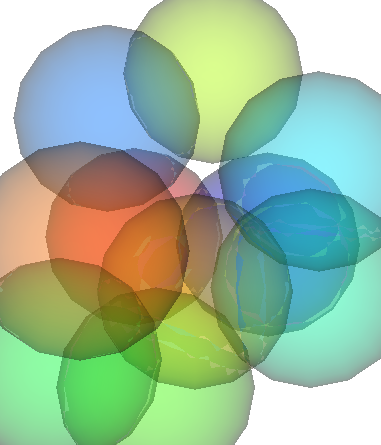
\includegraphics[height=2.0in]{./spheres_with_sort_crop.png}
 \end{center}
\end{minipage}
\begin{minipage}{0.28\textwidth}
 \begin{center}
 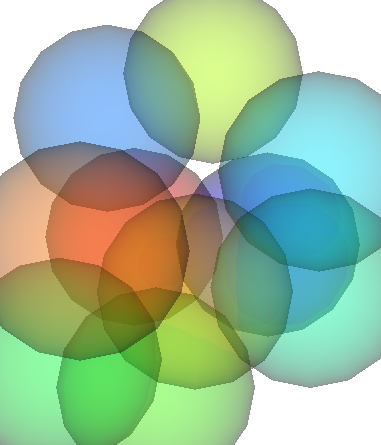
\includegraphics[height=2.0in]{./spheres_with_depth_peel_crop.png}
\end{center}
\end{minipage}
\begin{minipage}{0.3\textwidth}
 \begin{center}
 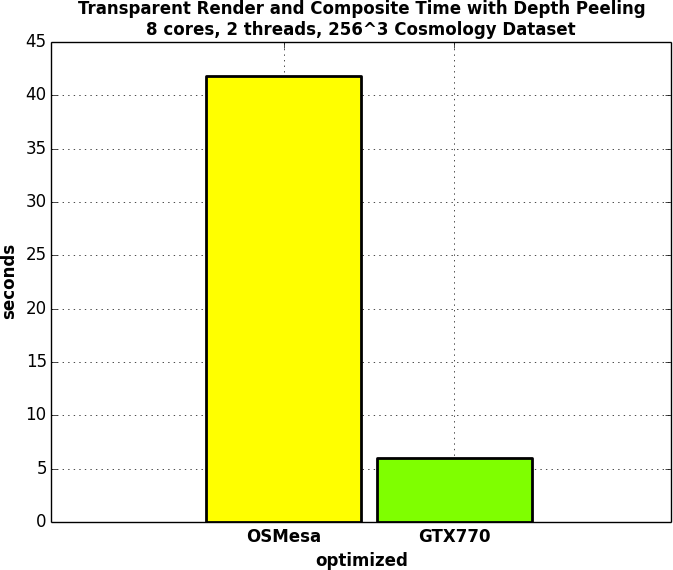
\includegraphics[height=2.25in]{./depth_peeling_time_cosmo.png}
\end{center}
\end{minipage}
\caption{\footnotesize {\bf Left:} Spheres rendered with camera order sort. {\bf Right:} Spheres rendered with depth peeling. {\bf Far Right:} Depth peeling performance.}
\label{fig:depth_peel}
\end{figure}
We investigated the use of depth peeling, a GPU accelerated algorithm that would eliminate the need for local camera order geometry sort during translucent rendering. In the implementation we tested there are two user modify-able parameters, number of peels and occlusion ratio. The occlusion ratio sets a threshold on the the fraction of pixels changed per peel below which the algorithm terminates. The number of peels sets the maximum number of peels to perform. When the occlusion ratio is set to zero all of the peels are performed. We found that for complex scenes 32 peels and a occlusion ratio of 0.01 were reasonable settings.  Unfortunately we found depth peeling to be substantially slower than the local geometry sort. The results are shown right most panel of figure \ref{fig:depth_peel}. 

Despite its poor performance depth peeling is a useful feature because VTK doesn't split intersecting geometry. The left two panels of figure \ref{fig:depth_peel} show a comparison of rendering using local geometry sort on the left and depth peeling on the right. Artifacts from intersecting geometry are present in the locally sorted rendering. Depth peeling is slower but produces the correct result. For this reason it is a useful feature to have available.

\section{VisIt integration:}
\begin{figure}
 \centering
 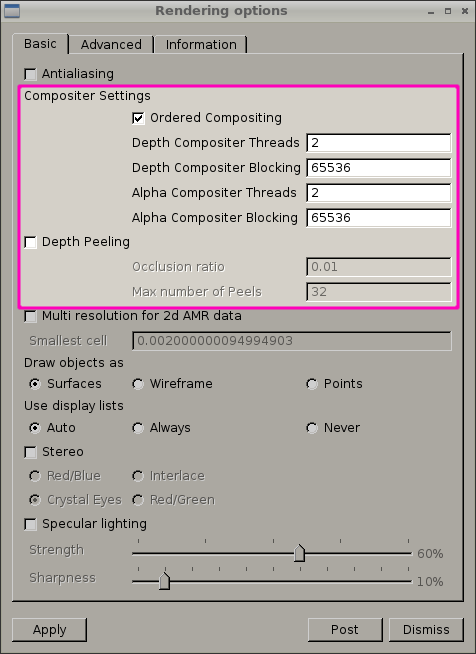
\includegraphics[height=3in]{./settings_window.png}
 \caption{Additions to VisIt's GUI controlling ordered compositing and depth peeling.}
 \label{fig:settings}
\end{figure}
We added controls in VisIt's GUI for the new features. These are shown in figure \ref{fig:settings}. Ordered compositing is enabled by default but can be optionally  disabled. Depth peeling is disabled by default be can be optionally enabled.

\section{Conclusion}
Compared to posthoc rendering, insitu rendering often generates larger numbers of images, as a result rendering performance and scalability are critical in the insitu setting. We implemented improvements to VisIt's rendering and compositing infrastructure that deliver increased performance and scalability in both posthoc and insitu settings. Specifically we have added alpha bend compositing capability to VisIt and applied the well known ordered compositing optimization for transparent rendering, and have addressed a number of performance issues. The impact is that VisIt performs is better prepared for insitu rendering work loads.

\end{document}